\chapter{Background}
\label{cha:background}
\section{VLSI and EDA}
\label{sec:VLSIalg}

The complexity of \glspl{ic} has been growing year after year since they were first introduced. According to Moore's Law \cite{moorelaw}, the density of transistors on a chip doubles approximately every 2 years. This tendency has been followed for the last 40 years, but of course such a fast-paced evolution of the number of transistors comes with a lot of challenges at many levels, such as technology, design and tools. \gls{vlsi} is the technology that allows combining millions of transistors in a single chip such as a microprocessor. This field has been constantly evolving, trying to make faster chips and integrate more transistors generation after generation. As the number of transistors has dramatically increased over the years, the complexity of circuits has also increased enormously; and with it, the challenges associated to the design of such circuits. \\

The design of \gls{vlsi} circuits is therefore a very complex process that requires automation. \gls{eda} is a category of software tools for designing electronic systems such as \glspl{ic}. This aid has been evolving together with the needs of \gls{vlsi} design since the mid-70s. Nowadays, given the level of complexity that \gls{vlsi} design has reached, \gls{eda} tools play a very important role in the fabrication of \glspl{ic}. \\

Current workflows for the fabrication of chips are very modular. The \gls{rtl} design abstraction, which models synchronous digital circuits and focuses on the flow of digital signals between hardware registers, is used to describe a circuit.  \glspl{hdl} such as Verilog and VHDL can be used to create such high-level representation of circuits. \gls{eda} tools are used to design and implement technology-dependent circuits from a higher level of abstraction. Automated synthesis goes through a lot of steps to transform an \gls{rtl} design into a geometrical layout, creating a physical design for the given \gls{rtl} specification. Given a high-level specification multiple final circuits can be considered valid, so there is room for a lot of decisions and optimization to be done in order to generate a good physical design of a circuit. \\

Given an \gls{rtl} circuit, these are some of the steps it goes through during the physical design phase. Note that all of these processes are automated by using the above mentioned \gls{eda} tools. We can consider that the output of one step is the input for the next one.

\begin{description}
  \item[Logic Synthesis] \hfill \\
  Given a circuit abstraction, such as an \gls{rtl} circuit, logic synthesis returns an implementation of the circuit in terms of logic gates. The \gls{rtl} design is translated into boolean expressions.  These formulas can be optimized using exact methods such as the Quine-McCluskey algorithm \cite{quine, mccluskey}, heuristic methods such as Espresso \cite{espresso} or kernel and boolean factorization. After these technology-independent steps, the formulas are mapped onto a given cell library resulting on a netlist in that technology library, using data structures such as \glspl{dag} and dynamic programming algorithms. To show a little example, this is a very simple module written in Verilog. \\ 
  

\begin{lstlisting}
module some_logic(a, b, c, out);
    input a, b, c, out;
    output out;

   assign out = (a & b) | c;

endmodule 
\end{lstlisting} 

Figure \ref{fig:some_circuit} represents the output of the logic synthesis phase receiving this code as an input. 
  
\begin{figure}[h!]
  \centering
  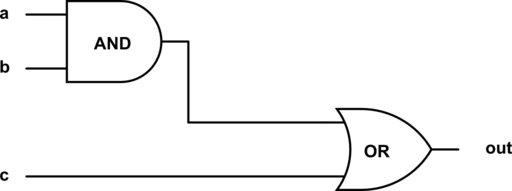
\includegraphics[scale=0.7]{img/bckgrnd/some_circuit.png}
  \caption{Logic gate level representation}
  \label{fig:some_circuit}
\end{figure}   
  
  \item[Floorplanning] \hfill \\
  This is the first step in the physical design flow. Floorplanning consists in identifying structures that should be placed close together, capturing relative positions rather than fixed coordinates. It can be considered a generalization of placement, a first draft of how things will be allocated in the chip, allowing transformations of the components such as rotations and modifying their shapes. Simulated annealing, trees and slicing structures, as well as dynamic programming for floorplanning optimization\cite{floorplan}, are widely used in this area. A floorplan can be optimized for metrics such as area, wirelength, routability and others. Figure \ref{fig:floorplan}, taken from \cite{changcheng}, shows two different floorplans for a given set of components. The floorplan on the left is optimal in area while the one in the right introduces white spaces.
  
\begin{figure}[h!]
  \centering
  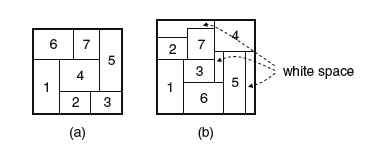
\includegraphics[scale=0.6]{img/bckgrnd/floorplan.png}
  \caption{(a) Optimal area floorplan (b) Non-optimal area floorplan}
  \label{fig:floorplan}
\end{figure}   
  
  \item[Partitioning] \hfill \\
  The netlist of the functions to implement can be very large. Partitioning is the process of dividing the chip into smaller blocks so that later placement and routing are easier, using a divide-and-conquer strategy to tackle design complexity. It is also a necessary step in the case of synthetisation on \glspl{fpga}, where a mapping from the netlist to hardware is needed. Many variants of partitioning exist, such as two-way partitioning (one of the first approaches, \cite{partitioning}), multi-way partitioning, which can be seen as an extension of the min-cut for two-way partitioning, and multi-level partitioning, where the result is represented by a tree structure. More partitioning approaches can be found in \cite{tutorialpartitioning}.
  
  \item[Placement] \hfill \\
  This step consists in assigning cells to positions in the chip according to some cost functions while preserving legality (for example, with no overlapping). The inputs are the netlists and the goal is to find the best position for each module considering wirelength, routability density, power and other metrics. Many placement styles exist depending on the design methodology it is integrated with (such as building blocks, standard cells or gate arrays). This step is tightly related to the next phase, routing. Some placement paradigms are:
  
	\begin{itemize}
 	 \item Constructive algorithms, such that when the position of a cell is fixed, it is not anymore modified. Some examples are cluster growth, min-cut \cite{placementprocedure}, or quadratic-placement algorithms (such as Hall placement \cite{hallplacer}, the first analytical placer).
 	 \item Iterative algorithms, where intermediate placements are modified in order to improve some cost function. This would include analytical methods such as force-directed placement. Figure \ref{fig:placement}, taken from \cite{changcheng}, shows several phases of the placement in a force-driven algorithm. The elements approach their final position iteration after iteration.
 	 \item Nondeterministic approaches, including metaheuristics like simulated annealing and genetic algorithms.
	\end{itemize}
	
  All these methods can be combined to obtain a more accurate result. Additionally other methods can be considered, for example a flow consisting of a global placement and legalization phase followed then by detailed placement step. There are many interesting research directions in placement such as manufacturability-aware placement, but probably the most interesting for our project would be routability-driven placement\cite{routabilitydrivenplacement}. More information about placement algorithms can be found in \cite{partitionchapter}.
  
\begin{figure}[h!]
  \centering
  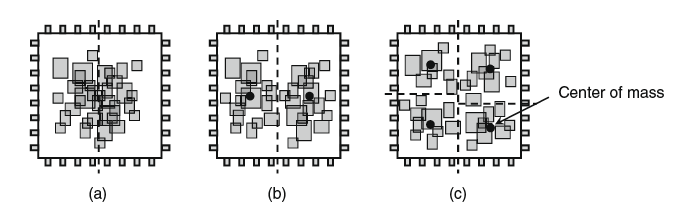
\includegraphics[scale=0.6]{img/bckgrnd/placement.png}
  \caption{Placement of a chip}
  \label{fig:placement}
\end{figure} 

  \item[Routing] \hfill \\
  The routing process determines the precise paths for nets on the chip layout, respecting a set of design rules to ensure that the chip can be correctly manufactured. It requires a physical placement of the layout, the netlists and the design rules required by the fabrication process. The main aim is to complete all required connections on the layout, although other objectives such as reducing total wirelenght or meeting timing requirements have become of essential relevance in modern chip design. The routing phase represents a very complex combinatorial problem. Usually, a two-step approach consisting of a global routing followed by a detailed routing is used. The first considers the connection between different regions of the chip, while the second focuses on obtaining a definite geometric layout for the wire connections.
\end{description}

These are only some examples of steps where algorithms have become indispensable for the design of \glspl{ic}. As we can see, \gls{eda} tools have become a basic component of digital circuit design. All of these steps have an important algorithmic load and much effort has been invested in such crucial synthesis tools. \\


\section{Cell Routing}
\label{sec:routing}


Routing is one of the multiple steps that take place in the physical design process. For the last years many algorithmic techniques have been explored to address the complex problem of determining how the components of circuits should be interconnected. As the number of transistors per chip grows, the increasing complexity of the design becomes a challenge for the routing stage. It is typically a very complex combinatorial problem that, as mentioned before, is usually solved using a two-stage approach: global routing and detailed routing. In this section we will overview both, as well as algorithms fitted for general routing. \\

\subsection{General Considerations}

The main aim of the routing problem is to find a valid interconnection of terminals that honors a set of design rules. Typically, most routing algorithms are based on graph-search techniques guided by parameters such as congestion and timing information, trying to find a balance of the net distribution among routing regions. For example, a chip might be partitioned into an array of tiles. Then the global router would find tile-to-tile paths for all nets on such a graph and use this information to guide the detailed router. \\

For the detailed routing step, two kinds of models exist: the grid-based and the gridless-based models. In the first, a grid is superimposed on the routing region and the detailed router finds routing paths in the grid. Gridless-based models, on the other hand, can use different wire widths and spacing. Even if they have more flexibility, grid-based routing is usually more efficient and easier to implement given its lower complexity compared to the other model. \\

When routing, two kinds of constraints appear: performance constraints and design-rule constraints. The objective of the performance constraints is to make connections meet the performance specifications provided by the chip designers. Design rules, on the other hand, are a set of additional constraints imposed by a given technology node that will have to be honored if we want the chip to be correctly manufactured. They impose restrictions on, for example, the minimum width of the wires or the wire-to-wire spacing. Another example of design rules is related to the layer models, which can be either \textit{reserved} or \textit{unreserved}. In the first case each layer is allowed only one routing direction, whereas the placement of wires with any direction is permitted in the other one.  Most of the routers, however, use the reserved model because it has lower complexity and is much easier for implementation; as we will see, manufacturability has a great impact on many of the decisions taken during the physical design flow. \\

\subsection{General-purpose Routing}

As mentioned before, graph-based algorithms have been extensively used for both global and detailed routing. In this section we will introduce the \textit{maze routing algorithm}, probably one of the most basic graph-search based algorithms. \\
 
Maze routing is based on a \gls{bfs}. Consider the grid on Figure \ref{fig:maze}. We want to connect the node marked with an $S$ to the one marked with a $T$. The grayed zones represent obstacles where the wire cannot be placed. \\

\begin{figure}[h!]
  \centering
  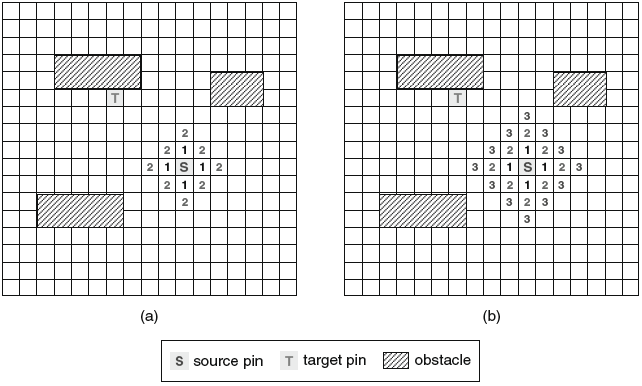
\includegraphics[scale=0.6]{img/bckgrnd/maze.png}
  \caption{Maze Routing - Wave Propagation}
  \label{fig:maze}
\end{figure} 

The maze router is composed of two basic steps: \textit{wave propagation} and \textit{retracing}. During the first step, starting from the source $S$, all adjacent nodes get labeled with a $1$, which is the distance from such nodes to $S$. In the next step, all cells adjacent to the nodes labeled $1$ get labeled with a $2$. This continues until the node $T$ is reached. We can see the wave propagation phase in Figure \ref{fig:maze} with the waves corresponding to $2$ and $3$. Once $T$ is reached, as seen in Figure \ref{fig:maze2}(a), a shortest path from $T$ to $S$ can be retraced by following any path such that the labels of the nodes decreases as shown in Figure \ref{fig:maze2}(b). Often, the preferred path is the one with the least number of detours. Notice that this algorithm guarantees to find the shortest path between two points if such a path exists. Both figures illustrating the example have been taken from \cite{changcheng}. \\

\begin{figure}[h!]
  \centering
  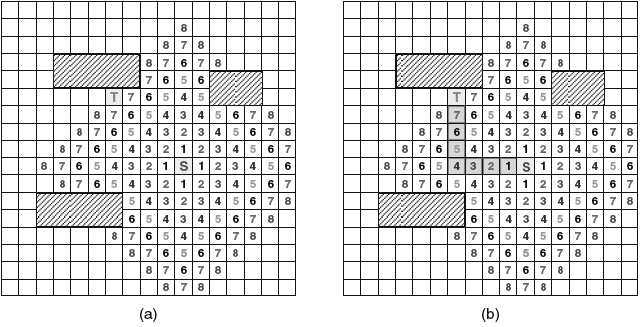
\includegraphics[scale=0.6]{img/bckgrnd/maze2.png}
  \caption{Maze Routing - Retracing}
  \label{fig:maze2}
\end{figure} 

This algorithm was proposed by Lee in \cite{lee} and is also widely known as \textit{Lee's Algorithm}. In practice, it is slow, memory consuming and difficult to apply to large-scale dense designs. Many methods have been proposed to reduce its running time and memory requirements. For example, alternative coding schemes for the nodes have managed to reduce the number of needed bits to merely two. Other variants include using depth-first search in combination with the \gls{bfs}, starting point selection or double fan-out. \\

After this algorithm, many other graph-based search algorithm appeared. The most significant ones probably are Line-search routing \cite{linesearch} and algorithms based on the well known A*-search proposed in \cite{astrella}, which are widely used in modern routers.

\subsection{Global Routing}
Global routing can be considered the most coarse grain type of routing. It consists in defining routing regions, generating tentative routings for nets and associating them to routing regions, but without specifying the actual layout of the wires. There exist two kind of global routing algorithms which differ on the basic routing strategy: sequential and concurrent algorithms. Whereas the first ones try to route signals one by one, concurrent algorithms try to find a valid solution for all signals at once. We will see a small introduction to each approach.

\begin{description}
  \item[Sequential global routing] \hfill \\
	In this schema we select a specific net order and then route nets sequentially according to that order. The quality of the solution greatly depends on the ordering given that an already routed net might block the routing of subsequent nets. Finding the optimal net ordering has been proven NP-hard. Often, a \textit{rip-up and re-route} heuristic is used to refine the solution. It basically consists in ripping-up some already connected nets and then re-route the ripped-up connections. It usually performs iteratively until all nets are routed, a time limit is exceeded or no gain is obtained. As we will see, CellRouter uses a similar heuristic to obtain better solutions once an initial legal routing has been found. The main drawback of this method is that, because of the dependence on net-ordering, if no feasible solution is obtained, it is not clear whether it does not exist or the chosen ordering was not good enough. 
  \item[Concurrent global routing] \hfill \\
	Concurrent global routing tries to establish all connections at the same time. Therefore, whether or not a solution is found does not depend on any net ordering. One of the most popular approaches is to model the layout as a graph and then use \textit{0-1 integer linear programming}. However, given it is NP-complete, another approach would be to solve the continuous \textit{linear programming} relaxation and the transform the fractional solution to integer solutions through a rounding scheme such as randomized rounding. In practice, such techniques are embedded into larger global routing frameworks which use a hierarchical, divide-and-conquer strategy. For routing multi-pin nets instead of two-pin nets, those multi-pin nets are usually decomposed using \textit{minimum rectilinear Steiner trees}.
  
\end{description}


\subsection{Detailed Routing}

The output of the global routing stage is used by the detailed router to determine the exact geometry of the nets in the chip. A popular type of detailed routing related to this project is full-chip routing. To cope with the scalability problem, routing frameworks use hierarchical and multilevel frameworks for large-scale designs. They use a divide-and-conquer approach by transforming large routing instances into smaller subproblems and later proceeding with a top-down, bottom-up or hybrid manner. In the first approach, the algorithm recursively divides the routing regions into smaller regions, routes the current level and refines the result in the next level. On the other hand, a bottom-up approach consists on initially partitioning the region into multiple small cells and, at each step, routing each region individually and merging it with its neighbors to form a larger supercell until the whole initial region is routed. The routing decisions made at any of the intermediate routing levels might be suboptimal, so hybrid approaches using both methods have also been explored. However, since routing decisions at a given level are irreversible, the quality of the solution is limited. This is a problem we will also face later in this project. \\

The same classification that we exposed for global routing algorithms can be applied to detailed routing algorithms. Sequential algorithms may not guarantee a solution even if it exists. For this reason, the most recent approaches tend to use concurrent routing. When doing detailed routing from a concurrent approach, two kind of algorithms can be considered, depending on the objects used to take routing decisions. \textit{Tree-based} algorithms first generate a set of candidate routing trees using algorithms that generate multiple \textit{minimum rectilinear Steiner trees}. Next, the problem is formulated as a multicommodity flow problem and solved as a 0-1 integer linear programming problem. On the other hand, \textit{segment-based} algorithms take decisions at the level of individual metal segments. This version has a finer granularity, at the expense of more computational complexity. However, manufacturing constraints are more easily represented in this scheme. Usually, SAT-based formulations are used to solve the routing problem under the segment-based approach. 
  
  
\subsection{Modern Routing}

It is interesting to consider the previous work directly related to the tool this project is based on. The closest is proposed in \cite{set}, a segment-based approach inspired by the satisfiability formulation presented in \cite{vuit}. However, \cite{set} only managed to route small gates given the high computational complexity of the resulting formulation, as will be shown in Chapter \ref{cha:cellrouter}. \\

As we have seen, many kind of routing strategies and approaches exist. It is not by sticking to one of the methodologies that routing can be easily solved. Given the complexity of the problem, many kinds of routers exist that combine several of the ideas briefly exposed in this short introduction to routing. For example, BoxRouter 2.0 \cite{boxrouter} is an academic global router that uses A*-search considering the congestion history of edges, wire rip-up and rerouting and finally a progressive integer linear programming approach to do layer assignment. The routing problem is constantly evolving and new algorithms and techniques will for sure continue to arise in order to meet with its new requirements. Fabrication considerations are day after day becoming more determining during the physical design process. \\

The figures for this section where taken from \textit{Electronic Design Automation: Synthesis, Verification, and Test}\cite{changcheng}. For more information on routing or VLSI algorithms in general, refer to at that book or to \textit{Handbook of Algorithms for Physical Design Automation}\cite{handbook}. \\


\section{Design Considerations}

When building digital circuits there exist multiple design styles, and the one used is chosen depending on the needs of the target design. Full-custom design is based on specifying the layout of each individual transistor and the interconnections between them. It potentially maximizes the performance and minimizes the area, but it is very laborious to implement. Full-custom design is typically used in a situation where there are area limitations or special application needs. Some examples are the design of cells within a standard cell library, memory cells or datapaths for high performance designs. However, other design methodologies exist. \\

\subsection{Standard Cell Design}

In the standard cell methodology, low-level \gls{vlsi} layouts are encapsulated in abstract logic representations (for example, as a NAND gate). This way, the logical level becomes independent from the physical level design. Using this design methodology, high-level design time becomes shorter as designs can be reused. Standard cell design relies on so-called standard cell libraries which contain primitive cells (such as AND or inverter) required for cell design. Additionally, more complex optimized cells can also be included. The cells in the library have a fixed height and variable width. This way they can be easily placed in rows easing the synthesis process. All cells on the row will be constructed according to a certain structure, for example the one shown in Figure \ref{fig:structure}. They are normally optimized full-custom layouts so that area and delay are minimized. \\

	
\begin{figure}[h!]
  \centering
  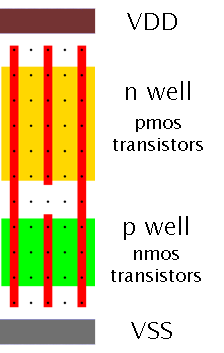
\includegraphics[scale=0.55]{img/bckgrnd/structure.png}
  \caption{Possible physical structure}
  \label{fig:structure}
\end{figure}


Each one of these cells is described by the following views. Additionally, metrics such as timing, power and noise for each cell are provided. 

\begin{description}

  \item[Logical View]  \hfill \\
	Cell's boolean logic formula, captured in a truth-table or boolean algebra equation, in the case of combinational logic, and a state transition table, in the case of sequential logic. Figure \ref{fig:logic1} is an example of a state transition table for an AND gate taken from the Nangate Cell Library documentation.
	
	
\begin{figure}[h!]
  \centering
  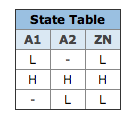
\includegraphics[scale=0.8]{img/bckgrnd/ANDlogic.png}
  \caption{AND gate, logical view}
  \label{fig:logic1}
\end{figure}

	
  \item[Schematic View]  \hfill \\
	Description of the transistors, their connections to each other and the terminals to the external environment. Multiple possible schematic representations for a given logical view exist. Figure \ref{fig:schematic1} is a schematic representation of an AND gate, also taken from the Nangate Cell Library documentation.
	
\begin{figure}[h!]
  \centering
  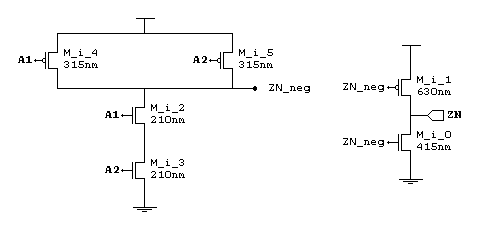
\includegraphics[scale=0.8]{img/bckgrnd/ANDschematic.png}
  \caption{AND gate, schematic view}
  \label{fig:schematic1}
\end{figure}

	
	
  \item[Layout View]  \hfill \\
	Physical representation of the cell. The most important from the manufacturing point of view, as it is the closest to the actual final design. Again, many possible layouts exist for a given schematic description of a cell. Figure \ref{fig:layout1} represents the layout of an AND gate.
	
\begin{figure}[h!]
  \centering
  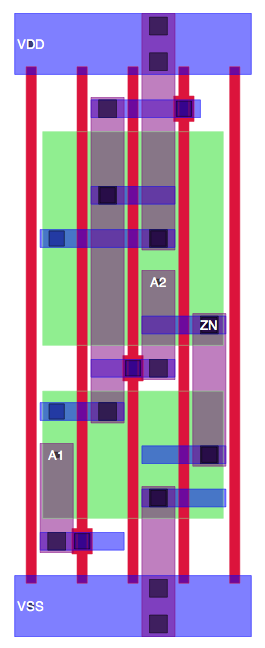
\includegraphics[scale=0.4]{img/bckgrnd/ANDlayout.png}
  \caption{AND gate, layout for schematic in Figure ~\ref{fig:schematic1} }
  \label{fig:layout1}
\end{figure}

\end{description}


Given the project works on the routing of standard cells, a simple method of representation of such cells has been chosen to illustrate important concepts in this report. It does not intend to be formal or exact, but useful as an abstraction to show situations that happen in real routing problem instances. Figure \ref{fig:celabase} shows an example of how one of these grids would look like. In such a 2D representation of a cell, all components sharing the same color are the ones that must be connected. When a terminal has no color, it means it is not important for what the figure intends to show so it is ignored. The voltage and ground signals are always on the top and the bottom of the cell. In this simple representation we will consider that wire segments can run along the columns and the indicated rows in the figure. 

\begin{figure}[h!]
  \centering
  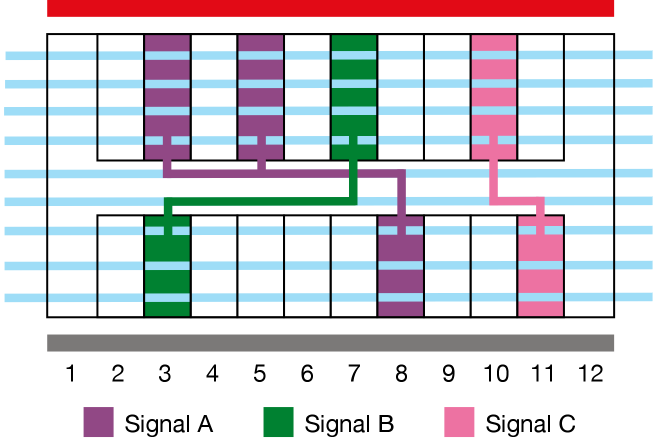
\includegraphics[scale=0.8]{img/bckgrnd/Celabase.png}
  \caption{An example of a cell representation}
  \label{fig:celabase}
\end{figure}



\subsection{Manufacturability-Aware Design}

As we have seen, standard cell design provides help by encapsulating primitives so that design becomes more modular and regular. However, in the last years additional problems have been adding up to the challenges of \gls{ic} design. As the size of transistors decreases, the manufacturing process has become increasingly complex. \\

One of the crucial processes involved in chip manufacturing is photolithography. During this process, chemicals which either harden or soften when exposed to ultraviolet light are used. Such products are applied onto the surface of the die and are exposed to light trough a mask with the desired pattern. After this step, the softened parts are removed and another mask with the next pattern is used. Layers grow one above the other until all masks have been applied. The patterns on the masks are the final product that the physical design produces for a given circuit abstraction. \\

This whole lithographic process is crucial to the fabrication of \glspl{ic}. Given the constant reduction in the size of the transistors as fabrication technology changes, the lithographic gap between such small component sizes and the light wavelength is having an increasingly important impact on the patterns used during the manufacturing process. Currently, \textit~{Resolution Enhancement Techniques} are applied to obtain transistor sizes much smaller than the light wavelength \cite{lithography}. Such approach is limited to a certain amount of geometrical configurations, contributing to an enormous increase of layout design rules at each technology generation. The design costs increases for two reasons. On one hand, the enormous effort required to verify such layouts. On the other hand, masks must be pre-distorted in order to compensate the distortions later introduced during the photolithography phase. \\

Litho-friendly layout techniques must be considered to deal with all this increasing complexity. These techniques exploit the use of one-dimensional features and gridded locations for layout elements. This complicates the design of standard cell libraries, that must now cope with such restrictions trying to provide the best possible area, performance and power consumption. However, using such techniques, manufacturability-aware physical layouts are produced, which are friendly to the fabrication process. \\

The aim of this project is to help in the synthesis of such manufacturability-aware standard cells. Today, it is a process where complex design rules are imposed. Given so, regularity has been introduced as a means to make design automation tractable. Such regularity can be seen for example in Figure \ref{fig:structure}, where a gridded layout is used. A clear example of such methodology can be found in \cite{LDP}, which proposes a model where all layout elements are located on a grid of evenly spaced points, with the grid unit begin a fraction of the wavelength of the light which will later be used during the fabrication process. As it will be explained later, the tools used in this project use a similar grid approach and try to be as technology-independent as possible, so that any desired design rule can be specified and the output of the tools is a physical design adapted to the desired technology constraints.


\section{Boolean Satisfiability Problem}
\label{sec:SAT}

As explained before, \gls{eda} tools rely on algorithms to tackle a variety of computational problems which arise during \gls{ic} design. One of the algorithmic problems that has attracted much attention during the last years has been the \gls{sat}. As we will see, much progress has been done and it can be used to face real industrial problems. For example, the routing tool used in this project is based on \gls{sat}.

\subsection{SAT problem}

First of all we will formalize the \gls{sat} problem and give some nomenclature that will be used in the later chapters. Suppose we have a set of \textit{variables},

\[ P = \{ p, q, r, \ldots \} \] 

We will define a \textit{formula} as follows.

\begin{enumerate}
  \item A variable is a formula.
  \item If $F$ is a formula, $\neg F$ is a formula.
  \item If $F$ and $G$ are formulas, $(F \wedge G)$ is a formula.
  \item If $F$ and $G$ are formulas, $(F \lor G)$ is a formula.
\end{enumerate} 

We will now define an \textit{interpretation} $I$ over $P$ as a map

\[ I \colon P \mapsto \{ 0,1 \} \]

It can be thought of as defining a value, either $0$ or $1$ (which can be read as \textit{false} or \textit{true}), to every variable in $P$. \\

We will also define the function

\[ eval_{I} \colon F \mapsto \{ 0,1 \} \]

as follows.

\begin{enumerate}
  \item $eval_{I}(p) = I(p)$
  \item $eval_{I}(\neg F) = 1 - eval_{I}(F)$
  \item $eval_{I}(F \wedge G) = min(eval_{I}(F), eval_{I}(G))$
  \item $eval_{I}(F \lor G) = max(eval_{I}(F), eval_{I}(G))$
\end{enumerate}

We will also consider that $I$ satisfies $F$ ($I \models F$) if $eval_{I}(F) = 1$. \\

For example, over the variable set $P$ that has been defined before, these would be well-constructed formulas.

\begin{itemize}
  \item $F_{1} = p$
  \item $F_{2} = r$
  \item $F_{3} = p \wedge q$
  \item $F_{4} = p \wedge \neg p$
  \item $F_{5} = (p \lor q) \wedge r$
\end{itemize}

Let us define an interpretation $I_{1}$ for $P$. \\

\begin{center}$I_{1}(p) = 1$, $I_{1}(q) = 1$, $I_{1}(r) = 0$\end{center} 

Under that interpretation, if we evaluate all five formulas we obtain

\begin{itemize}
  \item $eval_{{I}_{1}}(F_{1}) = eval_{{I}_{1}}(p) = 1$
  \item $eval_{{I}_{1}}(F_{2}) = eval_{{I}_{1}}(r) = 0$
  \item $eval_{{I}_{1}}(F_{3}) = eval_{{I}_{1}}(p \wedge q) = 1$
  \item $eval_{{I}_{1}}(F_{4}) = eval_{{I}_{1}}(p \wedge \neg p) = 0$
  \item $eval_{{I}_{1}}(F_{5}) = eval_{{I}_{1}}((p \lor q) \wedge r) = 1$

\end{itemize}

Now, let us define a \textit{model} to be an interpretation for which a given formula evaluates to 1. For example, $I_{1}$ is a model of $F_{1}$, whereas it is not a model of $F_{2}$. We will say that a formula is \textit{satisfiable} if it has at least a model, and we will say it is \textit{unsatisfiable} if there is no $I$ such that $eval_{I}(F) = 1$. In the case above, $F_3$ is clearly satisfiable, for $I_{1}$ is a model for it. On the other hand, $F_{4}$ is clearly unsatisfiable since, for any interpretation $I$, $p \wedge \neg p$ evaluates to 0. \\

The \gls{sat} problem now is straightforward to define. Given a formula, is there any interpretation that satisfies it? Or, in other words, is there any variable assignment such that the formula evaluates to 1? From the examples above, we can very easily see that all formulas except $F_{4}$ are satisfiable. \\

We will consider that any formula used as an input to \gls{sat} is in \gls{cnf}. First, let us define a \textit{literal} as a variable or the negation of a variable ($l_{1}, \neg l_{1}, l_{3}, \ldots$). Second,  let's define a \textit{clause} as a disjunction of literals ($l_{1} \lor l_{2}, \neg l_{1} \lor l_{3}, \ldots$). Now, we will say a formula is a \gls{cnf} if it is a conjunction of zero or more clauses, such as

\begin{center}$(l_{1} \lor l_{2}) \wedge (\neg l_{1} \lor l_{3}) \wedge (\neg l_{2} \lor \neg l_{3})$\end{center} 

Note that for a given $F$ there always exists a \gls{cnf} $G$ such that $G \equiv F$. \glspl{cnf} are used because the Tseitin Transformation \cite{tseitin} allows to obtain a \gls{cnf} from any arbitrary formula such that it is satisfied only by the interpretations that satisfied the original formula, with only a linear growth in size with respect to the original one. Solving the \gls{sat} problem for a formula in \gls{dnf}, which is defined as the \gls{cnf} but changing disjunctions for conjunctions and viceversa, would be achievable in linear time by scanning the clauses until a satisfiable clause appeared. However, no transformation such that an arbitrary formula is converted into a \gls{dnf} and avoids an exponential growth has been found. \\

It is important to note that \gls{sat} is NP-Complete, in fact the first one to be known \cite{cook}. Some restricted versions are known to be solvable in polynomial time, such as 2SAT and HORNSAT. However, even if it is NP-Complete, many practical instances can be solved in affordable time. Efficient and scalable algorithms for SAT developed in the last years have contributed to the use of SAT-solving engines as an essential tool in \gls{eda}.


\subsection{Using SAT}

The \gls{sat} problem is of central importance in many areas of computer science and industry. How can the \gls{sat} problem help in problems apparently as unrelated as industrial planning, scheduling of football leagues or the routing of standard cells? It is done by reducing a problem to \gls{sat}. \\

Consider a black-box SAT-solver, such that it receives a \gls{cnf} $F$ as an input and it returns ``YES'' if satisfiable, with a model that satisfies it, or ``NO'' otherwise. Reducing a problem to SAT consists on encoding our problem into a formula that we can give as an input to a SAT-solver in such a way that we can, in return, construct a solution to our problem from the answer the SAT-solver has provided. \\

The following example illustrates a simple reduction. We will use \gls{sat} to solve the $k$-CLIQUE problem. Given a graph of size $N$ and an integer $k$, $k$-CLIQUE returns ``YES'' if there is a totally connected subgraph of size $k$, ``NO'' otherwise. We will use the following variables.

\begin{center}$p_{i,j} =$ ``The $i$-th node in the graph is the $j$-th node in the clique''\end{center} 

Now we will explain how to construct a \gls{cnf} such that, if it is satisfiable we can get a k-clique from the graph, and there is no k-clique otherwise. We will have four groups of clauses.

\begin{enumerate}
  \item Every node in the clique must be at least one of the nodes of the graph. We can encode this clause as
  
  \begin{center}$p_{1,j} \lor p_{2,j} \lor \ldots \lor p_{N,j}$\end{center}  
  \begin{center}$\forall j, 1 \leq j \leq k$\end{center}
  
  \item Every node in the clique must be at most one of the nodes of the graph. We can encode this clause as
  
  \begin{center}$\neg p_{i,j} \lor \neg p_{i',j}$ \end{center} 
  \begin{center}$\forall i \forall i', i \neq i'$ \end{center} 
  \begin{center}$\forall j, 1 \leq j \leq k$ \end{center} 
  
  \item Every node in the graph cannot occupy two nodes in the clique.
  
  \begin{center}$\neg p_{i,j} \lor \neg p_{i,j'}$ \end{center} 
  \begin{center}$\forall j \forall j', j \neq j'$ \end{center}  
  
  \item For every two positions in the clique, if there is no edge connecting their nodes, they cannot both be in the clique.
  
  \begin{center}$\neg p_{i,j} \lor \neg p_{i',j'}$ \end{center} 
  \begin{center}$\forall i \forall i', i \neq i'$ and no edge between nodes $i$ and $i'$ \end{center} 
  \begin{center}$\forall j \forall j', j \neq j'$ \end{center}  
  
\end{enumerate}

Given an instance of $k$-CLIQUE, we can encode it in \gls{cnf} form. We use it as an input to a SAT-solver and examine its output. If it returns ``unsat'', it means that no assignment of values to the variables renders the formula true, thus implying that no clique of $k$ nodes exists. However, if it returns a model for the formula, by observing the $i$th index of the variables assigned to one we would be able to know which vertices are on the $k$-clique and which are not. \\

As we have seen, SAT can be used as a black-box tool to solve any problem that we can encode into a boolean formula. This approach is used by CellRouter. To solve the routing problem, we describe it in terms of a \gls{cnf} and use a SAT-solver to obtain a solution. There are many ways of creating such a formula and the success of this approach depends to a great extent on how variables are picked and restrictions are codified. However, as stated before, SAT is a supposedly difficult to solve problem. This approach is getting more attention because a lot of work is being done on the field, not only on SAT solving but in constraint programming (with examples such as Satisfiability Modulo Theories \cite{roberto}). Most modern SAT solvers are based on the DPLL algorithm, a systematic backtracking looking for a satisfiable assignment of the variables. However, a lot of additions and optimization have been added, such as conflict analysis, clause learning, backjumping, random restarts and heuristics. These methods have been proven empirically to be essential in solving large instances of SAT. For some more information on the use of SAT in EDA please refer to \cite{joao}. \\

\section{Conclusions}

This chapter has provided an overview of the key concepts this project is based upon. First the \gls{vlsi} design cycle has been introduced, with special emphasis on the use of \gls{eda} tools and algorithms. Then the routing problem has been presented, discussing about different algorithmic approaches that have been used to tackle the problem. Several design considerations that affect the fabrication process have been exposed, as well as a presentation to what a standard cell is and why it is important to \gls{vlsi} design. Finally, notions on what the boolean satisfaibility problem is and how it can be used to solve different problems have been given. Based on what has been shown, the next chapter will present the original framework this project is aiming to improve.